\documentclass[conference]{IEEEtran}
\usepackage[utf8]{inputenc}
\usepackage[T1]{fontenc}
\usepackage{amsmath,amssymb}
\usepackage{booktabs}
\usepackage{tikz}
\usetikzlibrary{arrows.meta,positioning,fit,backgrounds,calc}
\usepackage{xcolor}
\usepackage[colorlinks=true,allcolors=blue!60!black]{hyperref}

% palette (matches the project site)
\definecolor{cblue}{HTML}{2A78D6}
\definecolor{corange}{HTML}{EB6834}
\definecolor{cgreen}{HTML}{1BAF7A}
\definecolor{cink2}{HTML}{52514E}
\definecolor{cgrid}{HTML}{E1E0D9}
\definecolor{washblue}{HTML}{EAF2FC}
\definecolor{washgreen}{HTML}{E8F7F1}
\definecolor{washorange}{HTML}{FDF0EA}

\newcommand{\zcmd}{\ensuremath{z_{\mathrm{cmd}}}}
\newcommand{\snmr}{SNMR}

\title{Act Through the Latent: Toward a Learned\\Retarget-to-Track Interface for Humanoid Tracking}

\author{Anonymous ICRA Submission}

\begin{document}
\maketitle

\begin{abstract}
The dominant humanoid motion pipeline is two-stage: retarget human motion to the robot,
then train a tracking policy on the result. The interface between the stages is a stack
of robot-space joint targets---a representation chosen for convenience, not for control.
We take a first step toward a \emph{learned} interface. We distill a per-frame IK
retargeter into one multi-embodiment network with a shared retargeting latent
$z_{\mathrm{ret}}$ (128-d, five humanoids), and audit that latent with pre-specified
probes: it is instance-aligned across embodiments (window retrieval 57--83\% top-1 at
1.02\% chance---the low end is the morphological outlier; CKA 0.86--0.92), with motion
category not linearly decodable (0.151 vs 0.125 chance) though nonlinearly organized,
is embodiment-aligned but not invariant (0.28 linear probe vs 0.91 nonlinear attacker),
physically impoverished (contact F1 0.088 without supervision), and inert when
concatenated beside an explicit reference, a null that an independent ablation confirms.
On the control side we show a separate 64-d command code $z_{\mathrm{cmd}}$,
produced by a goal-conditioned residual-to-prior CVAE and DAgger-distilled from an
explicit-command RL teacher, can be the actor's \emph{only} motion input at $0.955\pm0.008$
ten-second completion versus the 0.98 teacher (3 seeds, 1{,}024 rollouts each). Feeding
the prior the frozen retargeting latent \emph{instead of} any robot-space reference
still reaches $0.656\pm0.044$ (mean survival 7.9 of 10\,s)---two-thirds of teacher
completion from a command channel computed purely from human motion---where a goal-free
prior collapses to 0.001 and
corrupting the latent collapses the arm to zero: the channel is necessary, not
bypassed.
The retargeting network also absorbs a second, interaction-rich teacher across three
human skeletons, cutting interaction-clip articulation error $3.1$--$5.2\times$ at
$+1.05$\,cm on locomotion (preliminary: ground-truth root). We release a pre-specified
negative-results ledger and two measurement defects---one in a widely used simulator
framework whose repair cut joint tracking error by 46\%, and one in our own trainer
whose repair \emph{overturned} our own published-internally negative on the frozen
latent, in our favor.
\end{abstract}

% ============================ FIGURE 1 ============================
\begin{figure*}[t]
\centering
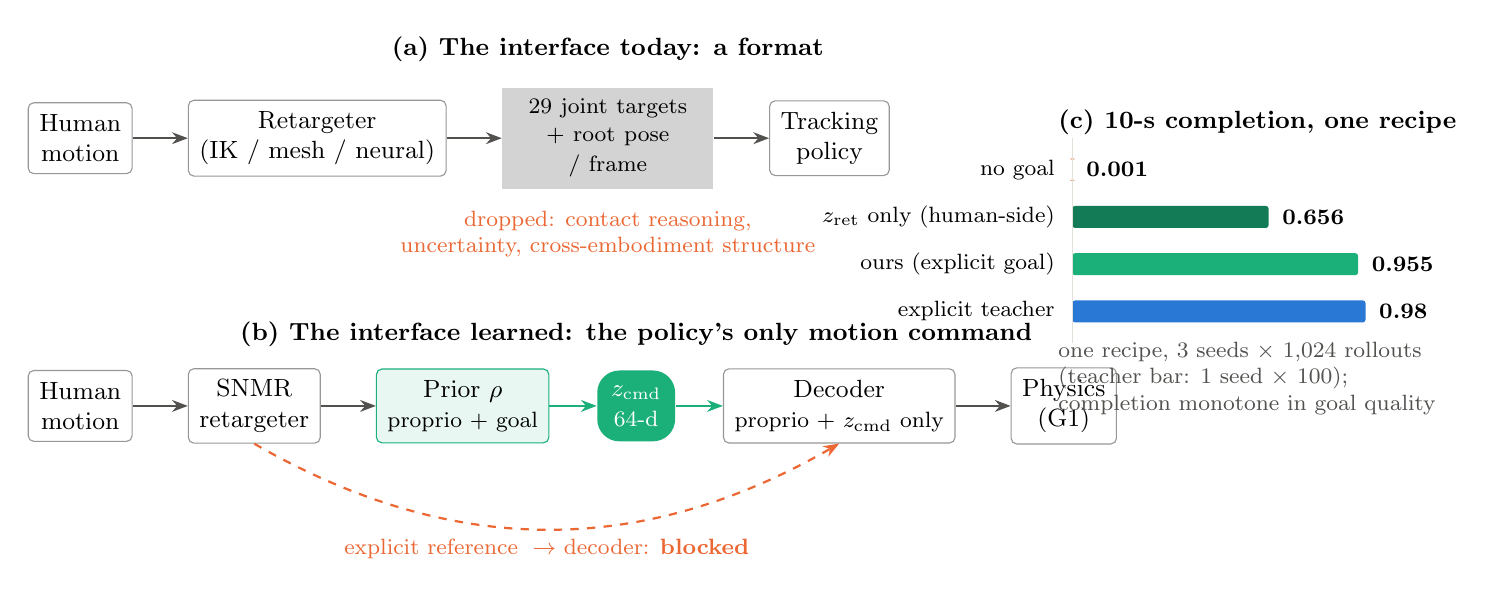
\begin{tikzpicture}[
  font=\small,
  node distance=4mm,
  box/.style={draw=cink2!60, fill=white, rounded corners=2pt, align=center,
              inner sep=4pt, minimum height=9mm},
  latent/.style={draw=none, fill=cgreen, text=white, rounded corners=8pt,
                 align=center, inner sep=5pt, minimum height=9mm},
  pipe/.style={draw=none, fill=cink2!25, align=center, inner sep=4pt, minimum height=9mm},
  arr/.style={-{Stealth[length=2mm]}, thick, cink2},
  blocked/.style={-{Stealth[length=2mm]}, thick, corange, dashed},
]
% ---------- panel (a): the interface today ----------
\begin{scope}
\node[box] (h1) {Human\\motion};
\node[box, right=7mm of h1] (r1) {Retargeter\\(IK / mesh / neural)};
\node[pipe, right=7mm of r1, text width=24mm] (p1) {\footnotesize 29 joint targets\\[-1pt]\footnotesize + root pose / frame};
\node[box, right=7mm of p1] (t1) {Tracking\\policy};
\draw[arr] (h1) -- (r1);
\draw[arr] (r1) -- (p1);
\draw[arr] (p1) -- (t1);
\node[below=1.5mm of p1, text=corange, align=center, font=\footnotesize]
  {dropped: contact reasoning,\\uncertainty, cross-embodiment structure};
\node[above=2mm of p1, font=\bfseries\small] {(a) The interface today: a format};
\end{scope}
% ---------- panel (b): the interface learned ----------
\begin{scope}[yshift=-34mm]
\node[box] (h2) {Human\\motion};
\node[box, right=7mm of h2] (r2) {\snmr{}\\retargeter};
\node[box, right=7mm of r2, fill=washgreen, draw=cgreen] (prior) {Prior $\rho$\\{\footnotesize proprio + goal}};
\node[latent, right=6mm of prior] (z2) {\zcmd\\{\footnotesize 64-d}};
\node[box, right=6mm of z2] (dec) {Decoder\\{\footnotesize proprio + \zcmd{} only}};
\node[box, right=7mm of dec] (sim) {Physics\\(G1)};
\draw[arr] (h2) -- (r2);
\draw[arr] (r2) -- (prior);
\draw[arr, cgreen] (prior) -- (z2);
\draw[arr, cgreen] (z2) -- (dec);
\draw[arr] (dec) -- (sim);
% the barrier: goal never reaches the decoder
\draw[blocked] (r2.south) to[out=-30,in=-150] node[midway, below, font=\footnotesize, text=corange]
  {explicit reference $\;\to$ decoder: \textbf{blocked}} (dec.south);
\node at ($(z2.north)+(0,4.5mm)$) [font=\bfseries\small] {(b) The interface learned: the policy's only motion command};
\end{scope}
% ---------- panel (c): the gap, measured ----------
\begin{scope}[xshift=125mm, yshift=-4mm]
\node[font=\bfseries\small, anchor=west] at (-2mm, 6mm) {(c) 10-s completion, one recipe};
% simple horizontal bar chart, hand-drawn
\foreach \y/\lab/\v/\c in {0/{no goal}/0.001/corange, -6/{$z_{\mathrm{ret}}$ only (human-side)}/0.656/cgreen!70!black, -12/{ours (explicit goal)}/0.955/cgreen, -18/{explicit teacher}/0.98/cblue}{
  \node[anchor=east, font=\footnotesize] at (0mm, \y mm) {\lab};
  \fill[\c, rounded corners=1pt] (1mm, \y mm - 1.4mm) rectangle ({1mm + \v*38mm}, \y mm + 1.4mm);
  \node[anchor=west, font=\footnotesize\bfseries] at ({1.5mm + \v*38mm}, \y mm) {\v};
}
\draw[cgrid] (1mm,-22mm) -- (1mm,4mm);
\node[font=\footnotesize, text=cink2, anchor=west, align=left] at (-2mm,-26.5mm)
  {one recipe, 3 seeds $\times$ 1{,}024 rollouts\\(teacher bar: 1 seed $\times$ 100);\\completion monotone in goal quality};
\end{scope}
\end{tikzpicture}
\caption{\textbf{The retarget-to-track interface, learned (single-clip scope; see
\S\ref{sec:limits}).} (a)~The standard humanoid
stack passes per-frame joint targets between retargeting and tracking, discarding the
retargeter's contact reasoning, its uncertainty, and the cross-embodiment structure it
learned. (b)~We replace that interface with a learned 64-d command latent: the goal
reaches the goal-conditioned prior but \emph{never} the decoder, so \zcmd{} is the
tracking policy's only motion command. (c)~Under one training regime (3 training seeds,
1{,}024 rollouts per evaluation), completion is monotone in what the prior sees: no goal
collapses (0.001), the frozen \emph{human-side} retargeting latent alone reaches 0.656,
the explicit robot-space goal 0.955, against the 0.98 explicit-command teacher.}
\label{fig:teaser}
\end{figure*}

\section{Introduction}

Nearly every humanoid that has learned to move from human motion has done so in two
stages: a retargeter converts human motion into robot-space joint trajectories, and a
reinforcement-learning tracking policy learns to follow them. The split is a good
engineering decision---retargeters and trackers are developed, evaluated, and reused
independently, and the recent generation of each is strong: interaction-preserving
optimization on the retargeting side~\cite{omniretarget}, physics-in-the-loop
retargeting~\cite{reactor}, and unified tracking controllers that follow thousands of
clips with one network~\cite{beyondmimic,gmt}. But the \emph{interface} between the
stages has escaped scrutiny. What actually crosses the boundary is a per-frame stack of
joint targets---a format, not a representation.

That format is lossy in three specific ways. It discards everything the retargeter knew
that is not a joint angle: its contact reasoning, its uncertainty, and the
cross-embodiment structure it learned when one network serves several robots. It is
evaluated by kinematic metrics (pose error, foot skate, penetration) that are blind to
\emph{trackability}---the GMR study~\cite{gmr} showed retargeting artifacts silently cap
what downstream RL can learn, evidence that the interface transmits harm as readily as
signal. And it is \emph{dimensionally unshareable}: a 29-DoF joint-target stream cannot
command a 23-DoF robot, so every multi-robot system pays the interface cost once per
embodiment.

The obvious repair fails, and the failure is informative. Handing the tracking policy the
retargeter's latent \emph{alongside} its usual reference does nothing: in our experiments
the policy ignores the latent (concatenation is null-to-harmful, $-10$ points at worst),
and UniTracker's ablation reports the same mechanism independently---``when the actor
receives the reference motion directly, the influence of the latent variable $z$
vanishes''~\cite{unitracker}. Training a latent by RL from scratch
collapses~\cite{unitracker,bfm}. But remove the explicit reference entirely, and the
picture inverts: fed to a co-trained prior as the \emph{only} goal source, the same
frozen latent carries two-thirds of the teacher's completion ($0.656\pm0.044$ vs 0.98)
where a goal-free prior collapses to 0.001. The retargeting latent is not inert; it is
\emph{dominated}---when a strictly more informative channel is available beside it,
the policy uses that channel and ignores this one.

\textbf{Our key insight is that the retargeting-to-tracking boundary should not be a
representation the two stages agree on, but one the tracking policy learns to act
through: a latent becomes useful for control exactly when it is the policy's only
channel to the goal, and is ignored whenever a more informative explicit reference is
available beside it.} The
sections that follow are the constructive and destructive halves of that claim. We build
\snmr{}, a skeleton-agnostic retargeting network distilled from a classical IK teacher
whose shared latent serves five humanoids, and we audit that latent with
falsification-first probes before asking it to do anything (\S\ref{sec:audit}). We then
make the interface load-bearing (\S\ref{sec:method}): a conditional VAE whose
goal-conditioned prior compresses the reference into a 64-d command latent, trained by
DAgger from an explicit-command RL teacher, with the reference visible to the prior but
never to the decoder. On a simulated Unitree~G1 this interface reaches
$0.955\pm0.008$ ten-second completion against its 0.98 teacher (Fig.~\ref{fig:teaser}c);
replacing the prior's robot-space goal with the frozen retargeting latent---so that
\emph{no robot-space reference exists anywhere in the student}---retains
$0.656\pm0.044$, and removing the goal entirely collapses to 0.001. The same latent then absorbs a second, interaction-rich
teacher---terrain and object clips from a fundamentally different retargeter, arriving on
different human skeletons---cutting interaction-clip error $3$--$5\times$ at a measured
$+1.05$\,cm locomotion cost (\S\ref{sec:exp}).

Two findings we did not go looking for became contributions. First, a world-body indexing
defect in a widely used MuJoCo-Warp training framework silently zeroed the primary
body-position tracking reward in every one of our runs (upstream report in preparation);
its repair cut
joint tracking RMSE by 46\% with no change to the learning algorithm and brought our
tracker into an externally calibrated band (\S\ref{sec:defect}). Second, rolling tracking
policies out on their own references and recording the simulated states yields physically
repaired supervision---$2$--$3\times$ less foot skate at a measured fidelity
price---quantifying the data-side alternative to physics-in-the-loop retargeting.

\textbf{Contributions.}
\begin{itemize}
\item \textbf{A learned command interface for humanoid tracking, under an exclusivity
  contract.} A goal-conditioned, residual-to-prior CVAE whose 64-d latent is the
  policy's only motion input---$0.955\pm0.008$ completion against a 0.98
  explicit-command teacher (3 seeds), with the reference never visible to the decoder
  and the code measurably a \emph{recoding}, not a copy (effective rank 14 of 64; the
  goal is less linearly decodable from \zcmd{} than from proprioception alone, held-out
  $R^2$ 0.48 vs 0.62); fed the frozen \emph{human-side} retargeting latent as its only
  goal source it retains $0.656\pm0.044$ (goal-free control: 0.001)---plus a documented
  failure anatomy (path consistency, goal conditioning, observation-layout leaks) for
  making such interfaces work.
\item \textbf{A falsification-first audit of a shared motion latent.} Pre-specified probe
  families establishing what the latent carries---instance-aligned, embodiment-aligned
  but not invariant, physically impoverished, dominated beside an explicit
  reference---with the negative verdicts stated as measured results, one independently
  replicated and one \emph{overturned by our own defect repair} (frozen-latent control
  value: from ``inert'' to two-thirds of teacher).
\item \textbf{Skeleton-agnostic retargeting distillation, measured honestly.} A
  1.5M-parameter network amortizing an IK teacher across five humanoids (limits by
  construction, 671\,fps CPU), and a separate two-teacher G1 study absorbing
  interaction-rich clips across three human skeletons at a quantified locomotion
  cost (preliminary: articulation under ground-truth root)---with the sharing cost and
  the zero-shot-embodiment failure ($5.2\times$) measured rather than assumed.
\item \textbf{A measurement-substrate defect, found, fixed, and released}, plus the
  pre-specified negative-results ledger---closed research lines with the evidence that
  closed them, so the field can stop re-deriving them.
\end{itemize}

\section{Related Work}
\textbf{Retargeting as preprocessing.} Classical retargeting solves per-frame IK with
hand-tuned correspondences~\cite{gmr}; interaction-mesh methods add hard contact
constraints~\cite{omniretarget}; ReActor moves retargeting inside physics via bilevel RL,
eliminating artifacts by construction~\cite{reactor}. All three families emit the same
interface---robot joint trajectories---and are evaluated by kinematic quality plus,
recently, downstream RL success~\cite{gmr,omniretarget}. None asks whether the
\emph{representation} handed to the tracker should itself be learned. Neural feed-forward
retargeters~\cite{ikmr,nmr,adamorph} amortize the optimization and, in AdaMorph's case,
span many embodiments through a morphology-agnostic latent---but their latents are
internal machinery, not command interfaces, and none is analyzed for what it carries.

\textbf{Tracking and its command spaces.} Modern trackers follow references specified as
joint targets with body-pose terms~\cite{beyondmimic,gmt,exbody2}; HOVER unifies multiple
command \emph{modes} by distillation~\cite{hover}; UniTracker compresses the reference
into a CVAE latent and is the closest precedent for our command interface---single-embodiment, with
no retargeter and no representation analysis~\cite{unitracker}. Latent skill spaces for
physics characters~\cite{pulse,maskedmimic,controlvae} establish the recipe elements we
verify at robot scale: learned conditional priors, residual-to-prior encoders,
distillation-not-RL. Behavioral foundation models~\cite{bfmzero} reach a promptable
latent from the opposite entry point---unsupervised RL with no retargeting anywhere. To
our knowledge no published system co-trains a \emph{multi-embodiment retargeting} latent
under the \emph{control} objective.

\textbf{Interface critiques.} BeyondMimic names a ``planning-control
gap''~\cite{beyondmimic}; the GMR study quantifies how retargeting quality caps
tracking~\cite{gmr}. Both stop at the boundary we cross: neither changes what the
boundary \emph{is}.

\section{The Two-Stage Interface}
\label{sec:interface}
A source motion $m_t$ enters a retargeter $R$; the standard interface hands the tracker
$\pi$ a reference $g_t = (q^{\mathrm{ref}}_t, \dot q^{\mathrm{ref}}_t)$ of robot joint
targets. We move the actor-visible reference behind a learned code:
$\zcmd = \mu_\rho(\mathrm{proprio}_t, g_t)$ (the current-frame command; a future window
is future work), under an \emph{exclusivity contract}: the goal is visible to the prior
$\rho$ and to the critic, but never to the decoder, so motion intent reaches the actor
only through the 64-d code. We use ``interface,'' not ``bottleneck'': the code is not
dimensionally narrower than the goal (64-d each), and no rate term constrains the
goal-to-code path---the claim is exclusivity and recoding, which we verify directly
(the deployed code has effective rank 14 of 64, and the goal is \emph{less} linearly
decodable from it than from proprioception, held-out $R^2$ 0.48 vs 0.62: the prior
discards reference detail and emits a control-sufficient code rather than a copy).
The prior's goal source is the experimental factor
(\S\ref{sec:exp}): the robot-space reference $g_t$ (the actor-side interface), the
source-side representation $z_{\mathrm{ret}}$ alone (the interface-replacement arm---no
robot-space reference anywhere in the student), both, or neither (control).

The latent's source is \snmr{}: a graph-attention encoder over the source skeleton
(per-node features, adjacency, global pooling---skeleton-agnostic by construction) maps
motion to a per-frame retargeting latent $z_{\mathrm{ret}}\in\mathbb{R}^{128}$
(distinct from the control code \zcmd{}); embodiment-conditioned graph
decoders (AdaLN on a 32-d embodiment code, $\tanh$ joint-limit heads) emit trajectories
for any of five humanoids. Trained by distillation from a per-frame IK
teacher~\cite{gmr} on 77 LAFAN1 clips $\times$ 5 robots (2.48M paired frames), it
reaches 3.66\,cm held-out MPJPE (CI $[3.46, 3.86]$; G1 specialist; 2.9--6.0\,cm shared
across all five robots) at 671\,fps on CPU, with zero joint-limit violations by
construction. Foot skate (0.29 vs teacher 0.05\,m/s) is the known inherited gap and is
treated as a measured limitation, not hidden.

\section{Auditing the Latent}
\label{sec:audit}
Before asking the latent to carry control, we measured what it holds. Four pre-specified
probe families, in increasing severity:

\textbf{Content: instance-aligned, not linearly semantic.} Cross-embodiment
\emph{window} retrieval hits 75--83\% top-1 at 1.02\% chance on four embodiments and
57\% on the fifth (the morphological outlier); CKA between per-robot encodings is
0.86--0.92. A \emph{linear} motion-category probe is near chance (0.151 vs 0.125), but
low-dimensional embeddings show clear category clusters: the structure is nonlinearly
organized, and we claim only that it is not linearly accessible---the same caveat we
apply to the embodiment probe below.

\textbf{Embodiment: aligned, not invariant.} A linear probe recovers the source
embodiment at only 0.28 accuracy, but a nonlinear attacker reaches 0.91---the classic
gap between ``not linearly decodable'' and ``absent.'' A height-normalization
intervention moves the attacker only $\sim$1\,pp, suggesting---though, being an
out-of-distribution intervention, not proving---that body scale is a minor share of
the leak.

\textbf{Physics: impoverished.} Foot-contact state is weakly present under pure
distillation: linear F1 0.088 at full budget---at the always-predict-contact baseline
for the label prevalence ($\approx$0.09), with AUROC 0.51--0.64 on the one
balanced-support clip, i.e.\ chance-level. A co-trained contact head injects it durably
(F1 0.227 at full budget, $1.8\times$ a deployable-heuristic baseline at 0.127) at a
real fidelity price ($+1.5$\,cm at loss weight 0.5), so physics enters the latent only
when supervised in.

\textbf{Control: dominated, not inert.} Concatenated beside the explicit
reference, the latent is ignored or harmful ($-10$\,pp)---when a more informative
channel to the goal exists, the policy takes it. Remove that channel, and the frozen latent alone
carries $0.656\pm0.044$ completion through a co-trained prior (\S\ref{sec:exp}). The audit is the
specification for \S\ref{sec:method}: the latent becomes an interface only when it is
made the sole channel and a prior is co-trained to read it.

% ============================ FIGURE 2 ============================
\begin{figure}[t]
\centering
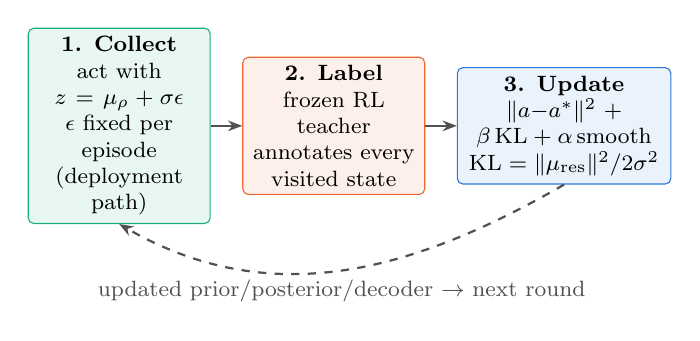
\begin{tikzpicture}[
  font=\footnotesize,
  box/.style={draw=cink2!60, fill=white, rounded corners=2pt, align=center, inner sep=3pt},
  arr/.style={-{Stealth[length=1.8mm]}, thick, cink2},
]
\node[box, fill=washgreen, draw=cgreen, text width=21mm] (collect)
  {\textbf{1. Collect}\\ act with $z=\mu_\rho + \sigma\epsilon$\\ $\epsilon$ fixed per episode\\ (deployment path)};
\node[box, fill=washorange, draw=corange, text width=21mm, right=4mm of collect] (label)
  {\textbf{2. Label}\\ frozen RL teacher\\ annotates every\\ visited state};
\node[box, fill=washblue, draw=cblue, text width=25mm, right=4mm of label] (update)
  {\textbf{3. Update}\\ $\|a{-}a^\ast\|^2 + \beta\,\mathrm{KL} + \alpha\,\mathrm{smooth}$\\ $\mathrm{KL} = \|\mu_{\mathrm{res}}\|^2/2\sigma^2$};
\draw[arr] (collect) -- (label);
\draw[arr] (label) -- (update);
\draw[arr, dashed] (update.south) to[out=-150,in=-30]
  node[midway, below, text=cink2] {updated prior/posterior/decoder $\to$ next round} (collect.south);
\end{tikzpicture}
\caption{\textbf{One DAgger round ($\times$2{,}000).} Rollouts are collected on the
deployment (prior) path with episodic noise; a frozen explicit-command teacher labels
visited states; the CVAE updates with action matching, a closed-form KL from the
residual-to-prior posterior (tied $\sigma$), and a latent smoothness term. The dashed
return edge makes it DAgger rather than behavior cloning. At deployment:
$\zcmd = \mu_\rho$ (deterministic), no teacher, no posterior, no explicit reference to
the actor.}
\label{fig:loop}
\end{figure}

\section{Making the Latent Load-Bearing}
\label{sec:method}
The method (Fig.~\ref{fig:loop}) is a conditional VAE trained by online distillation.
The \textbf{prior} $\rho(\zcmd \mid \mathrm{proprio}, g)$ sees deployable inputs only:
proprioception plus the reference goal window (and, in one arm, the frozen \snmr{}
latent stream). The \textbf{posterior} adds privileged simulation state as a
\emph{residual on the prior mean} with tied fixed $\sigma{=}0.3$, giving the closed-form
KL $\|\mu_{\mathrm{res}}\|^2/2\sigma^2$. The \textbf{decoder} maps
$(\mathrm{proprio}, \zcmd)$ to PD targets at 50\,Hz and never sees the goal. Training is
pure DAgger from a frozen explicit-command RL teacher (no RL gradient mixed in),
with episodic reparameterization noise and a latent smoothness regularizer.

Three failures fixed the design, in order. (i)~Collecting rollouts on the privileged
posterior path collapses deployment to 0.001 while the posterior path itself scores
0.84---train/deploy path consistency is not optional. (ii)~Mixing prior-path samples
into the action loss damages the posterior ($0.84\to0.42$) without rescuing deployment.
(iii)~Goal-conditioning the prior is the load-bearing fix, and a post-repair factorial
ablation gives the clean attribution: with a goal-conditioned prior, deployment reaches
$\approx$0.95 whether or not prior-path samples enter the action loss (the mix costs
2.3\,pp); without one, 0.000--0.002 either way. The working design compresses to one
line: \emph{the prior sees a goal; the posterior adds only a small privileged residual;
the decoder sees neither.}

\section{Experiments}
\label{sec:exp}
All tracking numbers: 10-second phase-stratified rollouts on a simulated Unitree~G1
(MuJoCo-Warp), deterministic deployment path, 1{,}024 rollouts per evaluation for latent
arms (100 for reference policies). \emph{Completion} is the fraction of rollouts that
track the full 10\,s without triggering the stack's standard tracking-failure
termination (anchor drift $>0.5$\,m or orientation error $>0.8$\,rad at any tracked
body, or end-effector deviation $>0.25$\,m)---i.e., a rollout ``completes'' only while
it stays within a bounded tube around the reference, not merely upright. Retargeting
numbers: 7 held-out LAFAN1 clips, bootstrap CIs over per-clip means. \emph{Recipe (for reproduction):} clip =
LAFAN1 walk1\_subject5; teacher = PPO, 8k iters at 512 envs with the repaired reward
stack plus a joint-space term ($w{=}1.0$, $\sigma{=}0.5$); students = 2{,}000 DAgger
rounds at 1{,}024 envs (24-step collection, 5 epochs, minibatch 4{,}096, Adam
$3{\times}10^{-4}$), prior/posterior MLPs $512{\times}256$, decoder
$512{\times}256{\times}128$, $\beta_{\mathrm{KL}}{=}0.1$, smoothness
$\alpha{=}0.005$, tied $\sigma{=}0.3$, goal = 58-d reference joints/velocities plus
6-d reference orientation. Code, protocol scripts with input hashes, and the
negative-results ledger accompany the submission.

\subsection{Does the learned interface work?}
Table~\ref{tab:main} is the paper's central result: a four-arm factorial over what the
prior sees, under one recipe (same DAgger algorithm, reward stack, budget, and seed;
1{,}024 rollouts per evaluation; all numbers post-repair of both defects in
\S\ref{sec:defect}). Completion is monotone in goal quality across completion, RMSE,
\emph{and} the imitation loss plateau (0.10/1.03/2.25 for explicit/$z_{\mathrm{ret}}$/no
goal). Three readings. First, the interface works: the 64-d command latent as the
actor's only motion input costs 2.5 points against its own teacher, where the design's
failed variants (posterior-path collection, goal-free priors) collapse to 0.001. An
attribution ablation confirms goal-conditioning is the load-bearing design choice: with
it, completion is $\approx$0.95 regardless of the action-loss sampling path ($-2.3$\,pp
for prior-path mixing); without it, 0.000--0.002 either way. Second, the frozen
retargeting latent alone---a channel computed purely from \emph{human} motion, with no
robot-space reference anywhere in the student---retains $0.656\pm0.044$, and two controls
constrain the interpretation: a goal-free prior collapses to 0.001 (the completion is
not gait-phase-from-proprioception), and corrupting the latent at deployment collapses
this arm to 0.000 on all three seeds (the channel is necessary---the prior did not
memorize the clip and route around its input). What these controls cannot yet separate
is goal \emph{content} from an exogenous \emph{clock}: on a single periodic clip,
phase information is nearly goal information, and the latent is fetched on the
reference's frame index. A matched-dimension phase-only control (a fixed random
projection of frame-index sinusoids through the identical fetch path) is registered
and queued; we report the substitution number with that caveat attached. Third, the remaining 30-point gap between
$z_{\mathrm{ret}}$-only and explicit-goal arms is the honest current price of removing
the robot-space reference; closing it (gradients into the retargeting encoder) is the
specified next step.

\begin{table}[t]
\centering
\caption{Command-interface factorial, one training regime (G1, walk1; mean$\pm$SD over
3 training seeds, 1{,}024 rollouts per evaluation).}
\label{tab:main}
\setlength{\tabcolsep}{4pt}
\begin{tabular}{lcc}
\toprule
Prior's goal source & Completion & RMSE \\
\midrule
--- (explicit-command teacher, bound)$^{\dagger}$ & 0.980 & 0.122 \\
Explicit robot-space command & $\mathbf{0.955\pm0.008}$ & 0.127 \\
Explicit cmd $+$ frozen $z_{\mathrm{ret}}$ & $0.956\pm0.003$ & 0.127 \\
Frozen $z_{\mathrm{ret}}$ only (human-side) & $0.656\pm0.044$ & 0.161 \\
No goal (proprio-only prior) & $0.001\pm0.001$ & 0.254 \\
\bottomrule
\end{tabular}

{\raggedright\footnotesize $^{\dagger}$single policy, 100 rollouts (reference-policy
protocol); no seed SD available.\par}
\end{table}

\subsection{Does the latent add value beyond the explicit goal?}
On single-clip walking: no---but it substitutes for most of it. The clean factorial
separates two questions the leak-era runs conflated. \emph{Additive} value beside the
explicit goal is null ($0.956\pm0.003$ vs $0.955\pm0.008$, paired per-seed deltas
straddling zero; the weaker of two redundant channels goes unused, consistent with
UniTracker's vanishing-influence observation). \emph{Substitutive} value is large:
$z_{\mathrm{ret}}$-only retains $0.656\pm0.044$ where the goal-free control collapses
to 0.001. The redundancy variant of the additive claim---the human-side latent should
buy robustness when the robot-space reference is corrupted---also fails on its first
valid test (the leak-era version noised dimensions the decoder never read): across
three seeds and three corruption levels ($1{,}024$ rollouts per cell), the paired gap
straddles zero at usable noise ($\sigma{\le}0.5$) and reaches only $+1.7$ to
$+4.1$\,pp where both arms are already broken ($\sigma{=}1.0$), below the
pre-specified $+5$\,pp gate---the second sub-gate trend our promotion discipline has
correctly rejected. The right reading of the interface program is therefore
substitution, not addition: the latent matters where an explicit command is
unavailable or unshareable---multi-clip and cross-embodiment settings, where a 29-DoF
target stream cannot command a 23-DoF robot at all. Those settings remain in progress:
multi-clip teachers at our compute budget have not yet cleared their quality gate
(0.47 mean completion at 1{,}024 envs $\times$ 16k iters over 8 heterogeneous clips;
the pre-registered 2{,}048-env retry is running).

\subsection{Does the interface scale with better retargeting data?}
\label{sec:twoteacher}
Preliminarily, yes (Table~\ref{tab:twoteacher}; articulation under ground-truth
root---object/terrain state is not yet input, and a redo with full root loss and
group-held-out splits is registered). Adding a second, interaction-rich
teacher---1{,}938 OmniRetarget clips~\cite{omniretarget} whose paired human data arrives
on 52- and 53-joint keypoint skeletons, ingested with MST-inferred topology and
synthetic orientations---cuts held-out interaction-clip error $5.2\times$ (object) and
$3.1\times$ (terrain) while locomotion pays $+1.05$\,cm. A sampling-diet ablation
attributes 61\% of the naive run's larger interference to data balance rather than
representational conflict. The dataset also delivers a measured lesson about
interaction multimodality: it contains 4{,}659 sibling pairs with \emph{bit-identical}
human motion and divergent robot trajectories (mean DoF divergence
0.031--0.068\,rad)---real conditional multimodality, $16$--$36\times$ the threshold
below which our earlier work showed generative decoders have nothing to model. We
tested whether conditioning explains it: a single terrain-scale scalar recovers 52\% of
terrain-sibling variance, but the exact per-frame 7-d object pose recovers only 6\% of
object-sibling variance under the same instrument. Terrain multimodality is
hidden-variable-explained; object multimodality (grasp-strategy choice, with arm
excursions up to 4.7\,rad between siblings) is not, so a deterministic decoder averages
modes on exactly the interaction-rich clips---the measured justification for a
generative decoding head, which we are testing under a pre-specified kill rule.

\begin{table}[t]
\centering
\caption{Two-teacher absorption, \emph{preliminary}: held-out articulation MPJPE
(cm) under ground-truth root pose; matched step budget.}
\label{tab:twoteacher}
\setlength{\tabcolsep}{4pt}
\begin{tabular}{lccc}
\toprule
Held-out pool & LAFAN1 & Two-tchr & $\Delta$ \\
\midrule
Locomotion (LAFAN1) & \textbf{3.31} & 4.36 & $+1.05$ \\
Object inter. & 28.95 & \textbf{5.53} & $-23.4$ ($5.2\times$) \\
Terrain inter. & 25.06 & \textbf{8.16} & $-16.9$ ($3.1\times$) \\
\bottomrule
\end{tabular}
\end{table}

\subsection{Are learned references as trackable as IK references?}
Matched tracking policies (3 seeds per source $\times$ 2 eval seeds $\times$ 100
rollouts) trained on \snmr{} references vs the IK teacher's: 86.7\% vs 86.7\%
completion---statistically indistinguishable (per-seed spread $\pm3$\,pp; the exact
tie is coincidence at this power)---with joint RMSE noninferior ($+0.33\%$,
CI $[-3.1, +4.9]\%$). This matrix predates the reward repair (\S\ref{sec:defect}); both sources trained
under the identical defect. A sensitivity control now validates the assay itself: a
tracker trained on a deliberately corrupted reference (i.i.d.\ joint noise,
$\sigma{=}0.05$\,rad --- the scale of known retargeting artifacts) drops to 0.48
completion against its own reference, a 46-point fall that is $9\times$ our
pre-specified detection gate. The completion assay is therefore sensitive to
reference-quality differences of the relevant magnitude, and the observed point-equality
is informative rather than an instrument blind spot. (The control's corruption is
i.i.d.\ while real retargeting error is spatially structured; a post-repair rerun on
harder clips remains registered.) Formal noninferiority on completion was not established: the
$\pm6$\,pp CI exceeds the pre-specified $-5$\,pp margin at this seed count---a power
statement, not a quality gap (per-seed spread $\pm3$\,pp dominates any source effect).

\subsection{What does physics-repaired supervision buy and cost?}
Rolling a calibrated tracker out on its own references and recording simulated states
yields repaired supervision with $2$--$3\times$ lower stance-foot speed than the
references themselves ($3$--$6\times$ on pre-repair policies) and zero penetration (a
simulator property, which we do not claim), at 6.2--6.7\,cm heading-local reconstruction
distance---the quantified data-side alternative to bilevel physics
retargeting~\cite{reactor}.

\section{A Defect in the Measurement Substrate}
\label{sec:defect}
While calibrating our tracker against external baselines we found that the primary
body-position tracking reward had been \emph{exactly zero} for every one of our
MuJoCo-Warp runs:
a world-body off-by-one (state tensors include the world body at index 0; the
body-name list excludes it) shifted every simulation-side body read one body rootward
in our stack (pinned revision; IsaacSim/IsaacGym paths unaffected), so the
tracked pelvis slot read the world body---always at the origin---and the exponential
reward kernel underflowed to 0.0 for 8{,}000 consecutive iterations (the raw term logs
show it). Policies still walked, because orientation and velocity terms survived; they
were orientation-plus-velocity trackers with a corrupted position channel. Repairing the
indexing (released as a small patch; IsaacSim/IsaacGym paths are unaffected, which is
why upstream never saw it) cut joint tracking RMSE from 0.263 to 0.142\,rad ($-46\%$)
with no change to the learning algorithm; adding a standard joint-space reward term then
reached 0.122\,rad at 0.98 completion, matching an external 187-run calibration band
(97.9\%). Paired comparisons made under the defect survive (both sources suffered
identically); absolute capability numbers did not. We report this at section level
because the lesson generalizes: \emph{measure your reward channels before tuning them.}

The same discipline then caught a second defect---in our own code. The observation
manager of our tracking stack concatenates observation terms \emph{alphabetically}, not
in configuration order; our distillation trainer sliced the explicit reference off the
front of the observation vector, where it is not. The consequence, established by causal
ablation (blanking the leaked dimensions at deployment drops completion from 0.93 to
0.00), is that in the affected runs the decoder saw the explicit reference inside its
``proprioception'' input, violating the exclusivity contract of \S\ref{sec:method}. All
interface-side numbers in this paper are from post-repair reruns; retargeting-side
results, the audit probes, the reference-policy baselines, and the trackability matrix
were never affected (their pipelines do not slice the observation vector). The repair
moved the results in \emph{both} directions: the explicit-goal arm improved
(0.935 to $0.955\pm0.008$---the corrupted goal slice had been hurting its prior), and
the frozen-latent-only arm went from 0.004--0.016 to $0.656\pm0.044$---under the leak,
the always-on explicit shortcut inside ``proprio'' suppressed learning from the latent
entirely, and a false negative we had logged as a closed research line reopened as this
paper's second result. The red flag that should have caught it earlier: under the leak, arms with
\emph{identical} goal information differed by ninety points of completion---an
incoherence input duplication cannot produce.

\section{Limitations}\label{sec:limits}
\textbf{Interface scope --- the central open step.} The $z_{\mathrm{ret}}$-only arm
reaches $0.656\pm0.044$ with a \emph{frozen} encoder; the 30-point gap to the
explicit-goal arm is unclosed, and the specified lever (tracking gradients into the
retargeting encoder) is queued. The latent's additive value beside an
explicit goal is null on single-clip walking; multi-clip and cross-embodiment
settings---where substitution is the only option---are in progress. \textbf{Embodiment generalization.} Zero-shot transfer to
an unseen robot fails ($5.2\times$ error); embodiment augmentation is the identified
path. \textbf{Physics of the latent.} Contact enters only by co-training at a fidelity
price; repaired references cost 6+\,cm at current tracker quality. \textbf{Interaction
tracking.} Our simulator path supports neither objects nor terrain in the tracking loop;
interaction data enters at the retargeting level only, where its absorption is measured.
\textbf{Simulation only.} No hardware; the MuJoCo-Warp stack is externally calibrated
but sim-to-real is unvalidated. \textbf{Data scale.} 4.6\,h/robot of locomotion plus
0.9--3.4\,h of interaction data is small; the two-teacher result is the first point on
the scaling curve, not its end. \textbf{Interaction multimodality is not yet modeled.}
Conditioning on the interaction hidden variable fails even given the exact per-frame
object pose (6\% of object-sibling variance recovered, vs.\ 52\% for terrain from a
single scalar)---deterministic decoding averages modes on precisely the
interaction-rich clips; a generative head with a pre-specified kill rule is under test.
Moving past these---closing the encoder-gradient gap, capacity scaling matched to data,
and the cross-embodiment command demonstration---is the immediate agenda.

\section{Conclusion}
The boundary between retargeting and tracking has been a file format. Treated as a
representation---audited before trusted, co-trained before deployed, and made the
policy's only channel to the goal---the learned code carries nearly everything the
explicit interface carried (0.955 vs 0.98), and the retargeter's own latent, computed
from human motion alone, carries two-thirds of it (0.656, with the clock-vs-content
control registered). The measurement lesson runs deeper than the architecture: this paper's
strongest results include a reward channel that was silently dead, a set of
pre-specified nulls, and a false negative of our own that only a defect repair
overturned; we commend all three practices---measuring reward channels, pre-specifying
gates, and hunting incoherence between arms---to the field.

\begin{thebibliography}{20}
\bibitem{reactor} D.~M{\"u}ller et al., ``ReActor: Reinforcement learning for
physics-aware motion retargeting,'' \emph{ACM TOG}, 2026.
\bibitem{omniretarget} L.~Yang et al., ``OmniRetarget: Interaction-preserving data
generation for humanoid whole-body loco-manipulation and scene interaction,'' arXiv:2509.26633, 2025.
\bibitem{gmr} J.~P. Araujo et al., ``Retargeting matters: General motion retargeting for
humanoid motion tracking,'' arXiv:2510.02252, 2025.
\bibitem{beyondmimic} Q.~Liao et al., ``BeyondMimic: From motion tracking to versatile
humanoid control via guided diffusion,'' arXiv:2508.08241, 2025.
\bibitem{gmt} Z.~Chen et al., ``GMT: General motion tracking for humanoid whole-body
control,'' arXiv:2506.14770, 2025.
\bibitem{unitracker} K.~Yin et al., ``UniTracker: Learning universal whole-body motion
tracker for humanoid robots,'' arXiv:2507.07356, 2025.
\bibitem{pulse} Z.~Luo et al., ``Universal humanoid motion representations for
physics-based control,'' \emph{ICLR}, 2024.
\bibitem{maskedmimic} C.~Tessler et al., ``MaskedMimic: Unified physics-based character
control through masked motion inpainting,'' \emph{SIGGRAPH Asia}, 2024.
\bibitem{controlvae} H.~Yao et al., ``ControlVAE: Model-based learning of generative
controllers for physics-based characters,'' \emph{SIGGRAPH Asia}, 2022.
\bibitem{hover} T.~He et al., ``HOVER: Versatile neural whole-body controller for
humanoid robots,'' \emph{ICRA}, 2025.
\bibitem{exbody2} M.~Ji et al., ``ExBody2: Advanced expressive humanoid whole-body
control,'' arXiv:2412.13196, 2024.
\bibitem{ikmr} X.~Chen et al., ``Implicit kinodynamic motion retargeting for
human-to-humanoid imitation learning,'' arXiv:2509.15443, 2025.
\bibitem{nmr} W.~Zhao et al., ``Make tracking easy: Neural motion retargeting for
humanoid robots,'' arXiv:2603.22201, 2026.
\bibitem{adamorph} H.~Zhang et al., ``AdaMorph: Unified motion retargeting via
embodiment-aware adaptive transformers,'' arXiv:2601.07284, 2026.
\bibitem{bfm} K.~Yin et al., ``Behavior foundation model for humanoid robots,''
arXiv:2509.13780, 2025.
\bibitem{bfmzero} Y.~Li et al., ``BFM-Zero: A promptable behavioral foundation model for
humanoid control using unsupervised reinforcement learning,'' arXiv:2511.04131, 2025.
\end{thebibliography}

\end{document}
